\section{Theory}
\begin{comment}
\textcolor{magenta}{\textbf{What must be clear by now
	 \begin{itemize}
	 	\item Consider case without covariates
	 	\item Make clear that SC is a weighted average of the donors
	 \end{itemize}}}
\end{comment}
In this chapter, we propose alternative \ac{SC}-estimators to assess the magnitude of treatment effects in observational settings. To establish a general basis, we first describe the contextual environment of the estimation. Similar to the setting as introduced by \ac{ADH}, we consider a framework with $J+1$ panel units indexed by $j = 0,1, ..., J$ that are observed over a time horizon of $T$ periods. Without loss of generality, assume that unit $j = 0$ is exposed to the treatment at period $t = T_0$ with $1 < T_0 < T$ and that there are no treatment anticipation and contamination (i.e., no spillovers in time and space). The former would be the case if the treatment affects unit $j = 0$ before $T_0$, the latter describes the case where some of the supposedly untreated units $j = 1,...,J$ are contaminated as they are affected by the treatment. To contextualize these assumptions, \cite{abadie:2010} argue that in the presence of anticipation effects, $T_0$ could be shifted back in time until the no anticipation assumption seem plausible. If panel units in the donor pool\footnote{To ensure direct comparability with the \ac{SC} literature, we adopt most of the commonly used terms. For example, control group units are labeled as 'donors'.} are affected by the treatment (contamination) as it is likely in the Brexit-application, those units could be removed from the sample prior to the estimation. Our goal is to evaluate the causal effect of the treatment, the specific functional form of which remains unspecified though. This is possible because the main goal of the \ac{SC}-estimation lies in the precise estimation of the counterfactual. Since the treatment  scenario is empirically observable, it is not necessary to specify the specific functional form of the it (e.g. level or slope shift, fading or persistent shock).

The following chapter is structured as follows: We first describe the canonical estimation procedure as proposed by \ac{ADH}. Furthermore, \ac{ADH} propose a model-invariant hypothesis testing approach. As this approach is employed in the further analysis, we also give a brief overview of these principles. Next we build intuition by considering a simple static scenario with only two donor units and one treatment unit. This setting is subsequently generalized to the case with more potential donors. The main difference between our extensions and the setting of \ac{ADH} is that we remove the weight constraints and that we analyze a situation without covariates. The former distinction guides us to the field of regularization to prevent our method from overfitting. The latter drastically reduces the data requirements and causes our algorithm to estimate the counterfactual with a significantly smaller information set. This fact leads us to the necessity of utilizing all available information and establishes our main contribution: The integration of  multivariate time series approaches into the \ac{SC}-algorithm. The theoretical derivation of this estimator completes the chapter.

\subsection{ADH Case}
We start by presenting the \ac{SC}-method and the testing procedure as introduced by \ac{ADH}. For the sake of comparability and due to its notational clarity, we borrow the employed notation of Abadie and colleagues. In terms of structural design, we build on the thorough presentation of the \ac{SC}-method and the related hypothesis testing procedure by \cite{firpo:2018}.

\textit{Setup} \\
The estimation task can be constituted by the potential outcome framework as introduced by \cite{neyman:1923} and elaborated by \cite{rubin:1974}. Let $y^{I}_{j,t}$ be the (potential) outcome for unit $j$ at point $t$ in the presence of the intervention. Likewise, let $y^{N}_{j,t}$ be the (potential) outcome for $j$ at point $t$ in the absence of the intervention. \ac{ADH} define the treatment effect of the intervention as 
\[
\delta_{j,t} = y^{I}_{j,t} - y^{N}_{j,t}
\] 
and introduce the indicator variable $D_{j,t}$ that takes on the value 1 if unit $j$ is treated at period $t$ and the value 0 otherwise. Given the assumed absence of anticipation and contamination, the following outcome is observed
\[
y_{j,t} + D_{j,t} \delta_{j,t} = 
\begin{cases}
	y^{N}_{j,t} &\text{(if } j = 0 \text{ and } t < T_0\text{)} \text{ or } j \geq 1, \\
	y^{N}_{j,t} + \delta_{j,t} &  \text{\phantom{(}if } j = 0 \text{ and } t \geq T_0
\end{cases}
\] 
The goal to estimate the causal treatment effect $(\delta_{0,T_0}, ..., \delta_{0,T})$ therefore boils down to the estimation of the counterfactuals of unit $j = 0$ in the post-treatment phase $(y_{0,T_0}, ..., y_{0,T})$, i.e. on what trajectory would unit $j=0$ have been, was there no intervention. The basic idea of \ac{ADH} is to estimate these counterfactuals as a weighted average of the donor outcomes using a data-driven approach to compute the weights. 
Intuitively, the weights are computed such that they optimally predict the outcomes and a set of time-invariant explanatory variables for the treatment unit in the pre-intervention phase, conditional on having a percentage interpretation. Thus, for the computation of the weights, we focus exclusively on the pre-intervention time periods $t \in \left\lbrace 1,2, ..., T_{0}-1\right\rbrace $. Subsequently, the counterfactuals are extrapolated by applying the calculated weights to the post-intervention time periods $t \in \left\lbrace T_{0},T_{0}+1, ..., T_{1}\right\rbrace $.

Let $Y_j = (y_{j,1}, ..., y_{j,T_{0}-1})^\prime$ be the vector of observed pre-intervention outcomes for unit $j$.\footnote{For instance, in the canonical example of \cite{abadie:2003}, $Y_0$ would be the vector of \ac{GDP}s for Great Britain until the Brexit referendum.} To distinguish treatment unit and donors, \ac{ADH} collect the treatment unit in the $((T_{0}-1) \times 1) $-vector $Y_0$ and row-bind all donor unit vectors into the $((T_{0}-1) \times J)$-matrix $Y_1$. Moreover, a set of $K$ time-invariant covariates of $Y_j$ is observed for all panel units.\footnote{In the already mentioned Brexit-example, natural predictors of \ac{GDP} are consumption, investment, government spending and net exports.} Therefore, let $X_0$ denote the $(K \times 1)$-vector of covariates for $Y_0$ and let $X_1$ denote the $(K \times J)$-matrix of explanatory variables for $Y_1$. To estimate the causal effect of the treatment, the \ac{SC}-estimator estimates the counterfactuals $(\widehat{y}_{0,1}, ...,\widehat{y}_{0,T_0},..., \widehat{y}_{0,T})$ of the single treated unit for the pre- and post-intervation phase as 
\[
\widehat{y}_{0,t} = \sum_{j = 1}^{J} \widehat{w}_j y^{N}_{j,t} \text{ } \forall \text{ } t \in \{1,...,T\}
\]
The weights $(\widehat{w}_1, ... , \widehat{w}_J)$ are constraint such that $\widehat{w_j} \geq 0 \text{ } \forall \text{ } j$ and $\sum_{j = 1}^{J} \widehat{w_j} = 1$. It is worth noting that this constraint requires the counterfactuals to belong to the convex hull of the donors as otherwise, $\widehat{Y}_{0}$ will never match its true counterpart. \cite{abadie:2010} argue that "the magnitude of discrepancy" should be calculated in advance of each \ac{SC}-application. If the researcher finds that the pre-intervention values of $\widehat{Y}_{0}$ fall outside the convex hull of the donors, the usage of \ac{SC} is not recommended. Formally, $(\widehat{w}_1, ... , \widehat{w}_J)$ is the solution of the following nested optimization problem:
%The weights $(\widehat{w}_1, ... , \widehat{w}_J)$ are obtained as the solution of a nested optimization problem that aims to match both the pre-treatment outcomes in $Y_0$ and the set of fixed pre-treatment covariates for the treatment unit in $X_0$. \ac{ADH} formalize this idea as follows
\[
\widehat{w}(v) = 
\underset{w}{\arg\min}
\sum_{k = 1}^{K} v_k \left(x_{0,k} - \sum_{j = 1}^{J} w_j x_{j,k} \right)^2 
\]
with $v$ being an arbitrary positive definite vector of dimension $(K \times 1)$ which solve the second optimization problem:
\[
\widehat{v} = 
\underset{v}{\arg\min}
\sum_{t = 1}^{T_0 - 1} \left(y_{0,t} - \sum_{j = 1}^{J}  \widehat{w}_j(v) y_{j,k} \right)^2
\]
Subsequently, the causal effect of the intervention $\delta_{j,t}$ can be quantified at each time point after the intervention $t \in \left\lbrace T_{0},T_{0}+1, ..., T_{1}\right\rbrace $ as the gap between observed ($y^{N}_{0,t} + \delta_{j,t}$) and predicted outcome ($\widehat{y}^{N}_{0,t}$).

This two-step estimation procedure serves two crucial purposes: $\widehat{v}$ measures the relative importance of the $K$ variables in $X_1$ to explain $X_0$. In contrast, the weighting vector $\widehat{w}(v)$ quantifies the relative importance of each unit in the donor pool. Summarizing the key concept of \ac{ADH}, the \ac{SC}-method ensures that the synthesized treatment unit is as similar as possible to the actual treatment unit with respect to the quantity of interest and a set of potential explanatory variables in the pre-treatment period. Especially in the canonical examples of \ac{SC}, the quantity of interest (e.g. \ac{GDP}) and the explanatory variables (e.g. consumption, investment, government spending and net exports) are interconnected by construction. Thus, observing that the \ac{SC}-estimator was capable of approximating both targets significantly enhanced the methods credibility. If explanatory variables are omitted, the \ac{SC}-algorithm reduces to an \ac{OLS} estimation, constraint to have no constant and weakly positive coefficients that sum up to one.
%The main concern when assessing treatment effects with the \ac{SC}-method in observational settings is the poor external validity of the estimation results for the post-treatment period. For example, especially when employing non-parametric statistical learning methods, it is simple to achieve a high in-sample (pre-treatment) fit. The crucial part when dealing with forecasts is that the observed in-sample patterns generalize well outside the verifiable horizon (post-treatment). One way to evaluate methods for detecting generalizable patterns is through hypothesis testing.

\textit{Hypothesis Testing} \\
The question of treatment effect significance arises naturally subsequent to the construction of the synthetic control. \ac{ADH} propose a model-invariant non-parametric inference procedure that is based on the Exact Hypothesis Test proposed by \cite{fisher:1971}. The basic idea behind such permutation tests is to compare the observed data with a number of randomly permuted versions of it, and to use the distribution of the test statistic calculated of the permuted samples to estimate the probability that the observed result occurred by chance alone. 

In the context of \ac{SC}, \ac{ADH} consider permutations in region (i.e. panel unit) and time. Region permutations estimate the treatment effect vector $(\delta_{j,T_0}, ..., \delta_{j,T})$ for each panel unit $j \in \{0, ..., J \}$.\footnote{Note that it is necessary to exclude the truly treated unit from donor pool to ensure the validity of the no contamination assumption.} This procedure provides the researcher with the empirical $(J+1)$-observational distribution of the treatment. Subsequently, it is possible to compare the estimated treatment vector $(\delta_{0,T_0}, ..., \delta_{0,T})$ of the truly treated unit with the $J$ placebo-treatment vectors of the units of the donor pool. Given the estimated treatment effect for $j=0$ is large, the null hypothesis of no treatment effect can be rejected at the significance level of one minus the percentile of $(\delta_{0,T_0}, ..., \delta_{0,T})$ in the empirical distribution.\footnote{For instance, let $J = 99$ such that treatment effects for 100 panel units can be computed. As long as the estimated treatment effect of the truly treated units belongs to the 95 largest effects (95th percentile or higher), the permutation test rejects the null hypothesis of no treatment effect at least at 5 percent.} Time permutations on the other hand consider only panel unit $j = 0$, permute $T_0$ to dates prior to the true treatment date and compute again the empirical treatment distribution. Given that $T_0 >> J$, this approach can increase the sensitivity of the test, since the theoretically feasible significance threshold of region permutation tests is determined by $\frac{1}{J}$. For both, region and time permutations, \ac{ADH} condense the vector of estimated treatment effects into a precision metric like the \ac{MSFE}\footnote{Note that \ac{ADH} speak of the Mean Squared Prediction Error for dates before and after $T_0$. Since we consider the time span until $T_0$ as prediction window and the time span after $T_0$ as forecast window, we employ the label \ac{MSPE} before $T_0$ and the label \ac{MSFE} from $T_0$ onward.} of the following form:
\[
MSFE_j = \frac{\sum_{t = T_0}^{T} \left(\widehat{y}_{j,t}^N - y_{j,t}^N\right) ^2}{T- T_0}
\]
A possible problem that can occur when assessing the relative rarity of the estimated treatment effect using the procedure described above is the existence of outliers in the donor pool. In the context of region permutations, suppose that a donor region is very different from the rest such that it falls outside the convex hull of the remaining donors. Note, that this circumstance does not cause problems for the truly treated region and its synthesized counterfactual as we expect the \ac{SC}-algorithm to assign a near zero weight to such an outlier. However, since the outlier itself cannot be synthesized precisely by the donor pool, both \ac{MSPE} and \ac{MSFE} are expected to be large. As this special feature causes the permutation test to be unreasonably conservative, \ac{ADH} propose to exclude regions who are hard to predict, i.e. who have a \ac{MSPE} that exceeds the \ac{MSPE} of the truly treated unit to a great extent. Figure \ref{F_01} visualizes the exclusion procedure in the tobacco control application of \ac{ADH}. 

\begin{figure}[H]
	\centering
	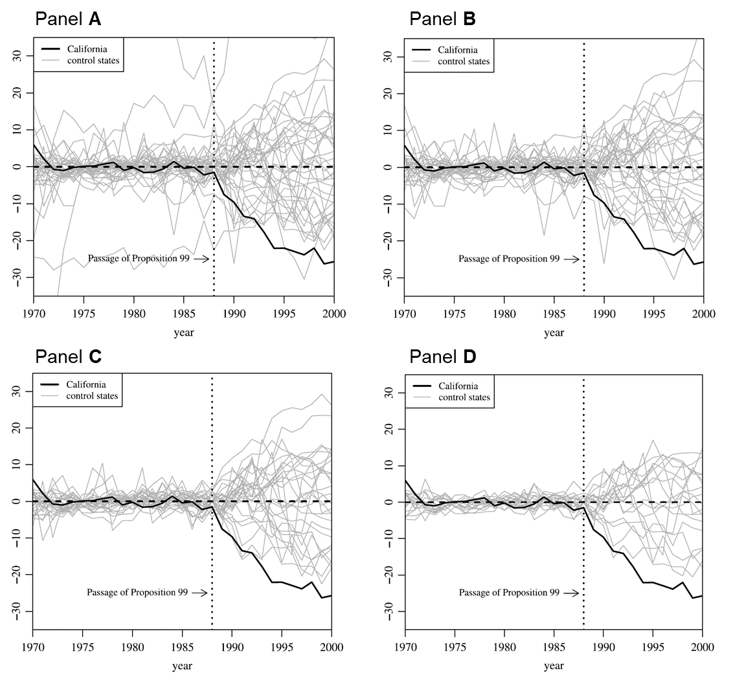
\includegraphics[scale=0.65]{F01}
	\caption{Region Exclusion Procedure of ADH}
	\label{F_01}
\end{figure}

The vertical axis indicates the gap between observed and estimated  per capita cigarette sales, the bold line represents the truly treated region (California). Two observations stand out when considering panel A: First of all, the treatment has a clear negative effect for California. Second, some regions have both a poor pre- and post-treatment fit. Since the treatment significance should not be artificially driven by regions with poor fit, \ac{ADH} successively remove regions with a large \ac{MSPE} relative to California. Panel B excludes regions with a \ac{MSPE} that is more than 20 times as large the \ac{MSPE} of California, Panel C lowers the cutoff to five times California's \ac{MSPE} and Panel D to  two times the \ac{MSPE}. In the last scenario, only 19 regions are left and California is the one with the most extreme treatment effect. The authors therefore conclude that the treatment is statistically significant with a (permutation) p-value of 5,3\% $\left(  \frac{1}{19} \right) $. 

One way to bypass the inefficient sample reduction procedure is to look at the distribution of the ratios of \ac{MSFE} and \ac{MSPE}. By scaling the post-treatment fit by the pre-treatment fit, regions with a poor fit are implicitly controlled for. In the tobacco control application, California is the region with the highest \ac{MSFE}-to-\ac{MSPE} ratio among all 39 regions which translates into a p-value of 2,6\% $\left(  \frac{1}{39} \right) $. 

\subsection{Simple Static Extension}
Once the fundamental framework of \ac{ADH} is established, we are prepared to introduce our proposed estimates. To give an intuitive introduction to our proposed extensions, we first consider the most simple scenario of one treatment unit $j = 0$ and two donor units $j = 1,2$. We consider a setting where only the outcome series (e.g. \ac{GDP}) and no further covariates (e.g. consumption, investment etc.) are observed. It is assumed that before $t = T_0$ the units have a joint distribution of the form 
\[
Y = \begin{pmatrix} y_0\\ y_1\\ y_2 \end{pmatrix} \sim \mathcal{N}(\mu,\Sigma)
\text{ for } t<T_0.
\] 
with $\mu = \left(\mu_0, \mu_1, \mu_2  \right)^\prime$ and the positive definite covariance matrix
\[
\boldsymbol{\Sigma} = \begin{pmatrix} \sigma_0^2 & \boldsymbol{\sigma_{12}^\prime} \\
	\boldsymbol{\sigma_{12}} & \boldsymbol{\Sigma_2} \end{pmatrix}.
\] 
$\sigma_0^2$ denotes the variance of $y_0$, $\boldsymbol{\Sigma_2}$ is a $(2 \times 2)$ covariance matrix of the vector $(y_1, y_2)^\prime$ and $\boldsymbol{\sigma_{12}}$ is a $(2 \times 1)$ vector with elements $cov(y_0, y_1)$ and $cov(y_0, y_2)$.

Disregarding any constraints, we are interested to derive the best unbiased forecast of $y_0$ given the controls $y_1$ and $y_2$ which is obtained as
\begin{equation*}
	\begin{split}
		\widehat{y}^{N}_{0} & = \mu_0 + w_1^{OLS} (y_1 - \mu_1) + w_2^{OLS} (y_2 - \mu_2) \\
		& = \mu^* + w_1^{OLS} y_1 + w_2^{OLS} y_2
	\end{split}
\end{equation*}
where $\mu^* = \mu_0 - w_1^{OLS} \mu_1 - w_2^{OLS} \mu_2$. This forecast can be directly estimated by an unrestricted \ac{OLS} regression of $y_0$ on $y_1$ and $y_1$. However, the result implies that there is no inherent reason to impose the restrictions that $w_1^{OLS}, w_2^{OLS} \geq 0$ and $w_1^{OLS} + w_2^{OLS} = 1$. Furthermore, we argue that the construction of \ac{SC} should include a constant term, as otherwise the estimated counterfactual may have a mean outside the convex hull of the donor means. See also \cite{doudchenko:2016} for a careful discussion of these restrictions. 

For illustrative reasons, assume that 
\[
Y \sim \mathcal{N}\left( 
\begin{pmatrix} 1\\ 1\\ 1 \end{pmatrix}, 
\begin{pmatrix} 1 &0.1 &0.4\\0.1 &1 &0.5\\0.4 &0.5 &1 \end{pmatrix}\right). 
\] 

For this example the unrestricted optimal weights for the counterfactual result as $w_1^{OLS} = -0.1333$, $w_2^{OLS} = 0.4667$ and $\mu^* = \mu_0 - w_1^{OLS} \cdot \mu_1 - w_2^{OLS} \cdot \mu_2 = 0.6667$.\footnote{The derivation of the employed estimators is postponed to the appendix.} Note that $w_1^{OLS}$ is negative even though all bivariate correlations between the units are positive. One may argue that this result does not make much sense as the economic interpretation of $y_1$ entering the counterfactual $\widehat{y}^{N}_{0}$ with a negative sign is unclear. This demonstrates the trade-off between optimality in a statistical sense and the economic interpretation of the solution.  

What happens if we impose the restrictions that all weights are positive and sum up to unity? In this case the restricted optimum yields the linear combination $\widetilde{y}^{N}_{0} = 0.2 y_1 + 0.8 y_2$.
The important difference lies in the variance of these estimates. For our example we obtain
\begin{equation*}
	\begin{split}
		& var(y_0 - \widehat{y}^{N}_{0}) = 0.8267 \\
		& var(y_0 - \widetilde{y}^{N}_{0}) = 1.1600.
	\end{split}
\end{equation*}
It is interesting to note that the variance of the restricted estimate is even larger than the unconditional variance of $y_0$. This is possible as $(w_1, w_2) = (0,0)$ is not included in the restricted parameter space. 

So far we argued and showed illustratively, that an unrestricted \ac{OLS} estimate can be superior to the constraint \ac{SC} estimate in settings with few panel units and a clear correlation structure among the units. This indication will be further refined in subsequent Monte Carlo simulations. In microeconometric settings it is usually assumed that the units in the treatment group and units in the control group are uncorrelated. In such cases the construction of a \ac{SC} is unpromising as the dependency between treatment unit and donors is the core condition for a plausible estimation of the counterfactual. In macroeconomic applications however, the variables in the treatment and control group (e.g. \ac{GDP}) are typically correlated and it is therefore important to model this relationship. As the simple scenario with only two panel units in the donor pool is highly unrealistic in practice, we now move to the general static case with $J+1$ panel units.
\subsection{General Static Extension}
In empirical macroeconomic practice, the quantities of interest are commonly measured at monthly or quarterly intervals, typically not at a coarser resolution. Hence, it is frequently observed that the number of pre-intervention time periods ($T_0 - 1$) is relatively small and may even be smaller than the number of units in the donor pool $J$. In such scenarios, the unrestricted \ac{OLS} estimate may face issues of instability or, in the case of $T_0 - 1 < J$, due to singularity, it may not even be identified. \ac{ADH} solve this issue by restricting the weights to be non-negative and to sum up to one. This regularization is essential as it prevents the method from overfitting the pre-treatment data and guarantees the existence of unique weights, especially when dealing with a small number of pre-treatment periods. However, alternative methods are also capable of ensuring weight stability and generalizability. For example, \cite{doudchenko:2016} suggest using an elastic net regression to regularize the donor weights and obtain comparable estimated treatment effects for different empirical applications of \ac{SC}. Their objective function has the following form:
\[
\widehat{w} = 
\underset{w}{\arg\min}
\sum_{t=1}^{T_0-1}\left(y_{0,t} - \mu^* - \sum_{j = 1}^{J} w_j y_{j,t} \right)^2 + 
\lambda_1 \left( \sum_{j = 1}^{J} w_j^2 \right) + 
\lambda_2 \left( \sum_{j = 1}^{J} |w_j| \right)  
\]
there are also other competing procedures to ensure weight stability and generazibility like the elastic net for synthetic controls as proposed by . 

Therefore some kind of regularization is necessary to obtain a reliable estimate of $\widehat{Y}_0^N$. 

\begin{equation*}
	Q(w, \lambda_1, \lambda_2) = \sum_{t=1}^{T_0-1}\left(y_{0,t} - \mu^* - \sum_{j = 1}^{J} w_j y_{j,t} \right)^2 + 
	\lambda_1 \left( \sum_{j = 1}^{J} w_j^2 \right) + 
	\lambda_2 \left(1- \sum_{j = 1}^{J} w_j
	 \right)  
\end{equation*}
\subsection{Univariate Dynamic Extension}

\textcolor{magenta}{\textbf{What must be clear by now
		\begin{itemize}
			\item TBD
\end{itemize}}}
When modeling macroeconomic time series it is often assumed that the $(k+1)\times 1$ vector of time series $y_t = (Y_{0t}, ..., Y_{kt})^\prime$ can be represented by a \ac{VAR} model given by 

\subsection{Multivariate Dynamic Extension}